\chapter{算例分析}
\label{cha:Example}

\section{算例}

设想一个四节点机组网络有向图如图~\ref{fig:Directed-graph}:

%去除Visio白边:http://www.mamicode.com/info-detail-2181323.html

\begin{figure}[htbp] % use float package if you want it here
    \centering
    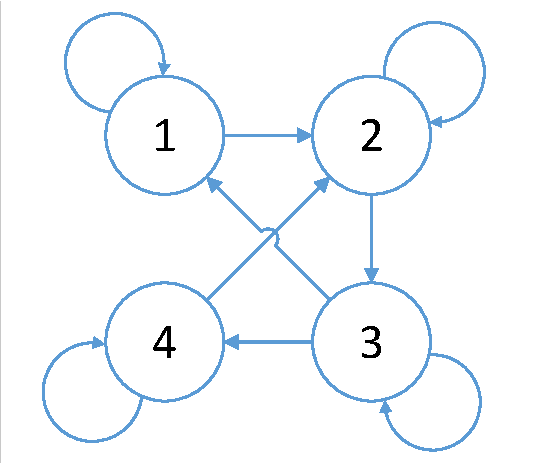
\includegraphics{Directed-graph.pdf}
    \caption{四节点机组网络有向图}
    \label{fig:Directed-graph}
\end{figure}

各节点处机组参数与负荷如表~\ref{tab:example}:

\begin{table}[htbp]
    \centering
%    \resizebox{\textwidth}{!}{%
    \begin{tabular}{@{}ccccc@{}}
    \toprule
    \multicolumn{1}{c}{Node} & $\alpha_{i}(\mathrm{MW})$  & $\beta_{i} \quad\left(\mathrm{MW}^{2} / \mathrm{S}\right)$ & $\gamma_{i}(\mathrm{S})$   & $L_{i}(\mathrm{MW})$    \\ \midrule
    1                        & -1 & 1 & 0.2 & 15.5 \\
    2                        & -2 & 2 & 0.1 & 0    \\
    3                        & -3 & 3 & 0.5 & 15.5 \\
    4                        & -1 & 2 & 0.7 & 0    \\ \bottomrule
    \end{tabular}
%    }缩放表格(字会变得很大)
    \caption{4节点算例机组参数与实时负荷}
    \label{tab:example}
\end{table}

其邻接矩阵为:

\begin{equation}
    A=\left[\begin{array}{cccc}
    {1} & {1} & {0} & {0} \\
    {0} & {1} & {1} & {0} \\
    {1} & {0} & {1} & {1} \\
    {0} & {1} & {0} & {1}
    \end{array}\right]
\end{equation}


\section{简化后的平均值共识算法}

运行附录~\ref{sec:Consensus}中的Python3脚本我们可以得到:

简单取平均后得到过渡矩阵为

\begin{equation}
    Q=\left[\begin{array}{cccc}
    {\frac{1}{2}} & {\frac{1}{2}} & {0} & {0} \\
    {0} & {\frac{1}{2}} & {\frac{1}{2}} & {0} \\
    {\frac{1}{3}} & {0} & {\frac{1}{3}} & {\frac{1}{3}} \\
    {0} & {\frac{1}{2}} & {0} & {\frac{1}{2}}
    \end{array}\right]
\end{equation}

取初值为1,2,3,4迭代10次:

随着迭代各机组的价格曲线如图~\ref{fig:Result-1234}所示。

\begin{figure}[htbp] % use float package if you want it here
    \centering
    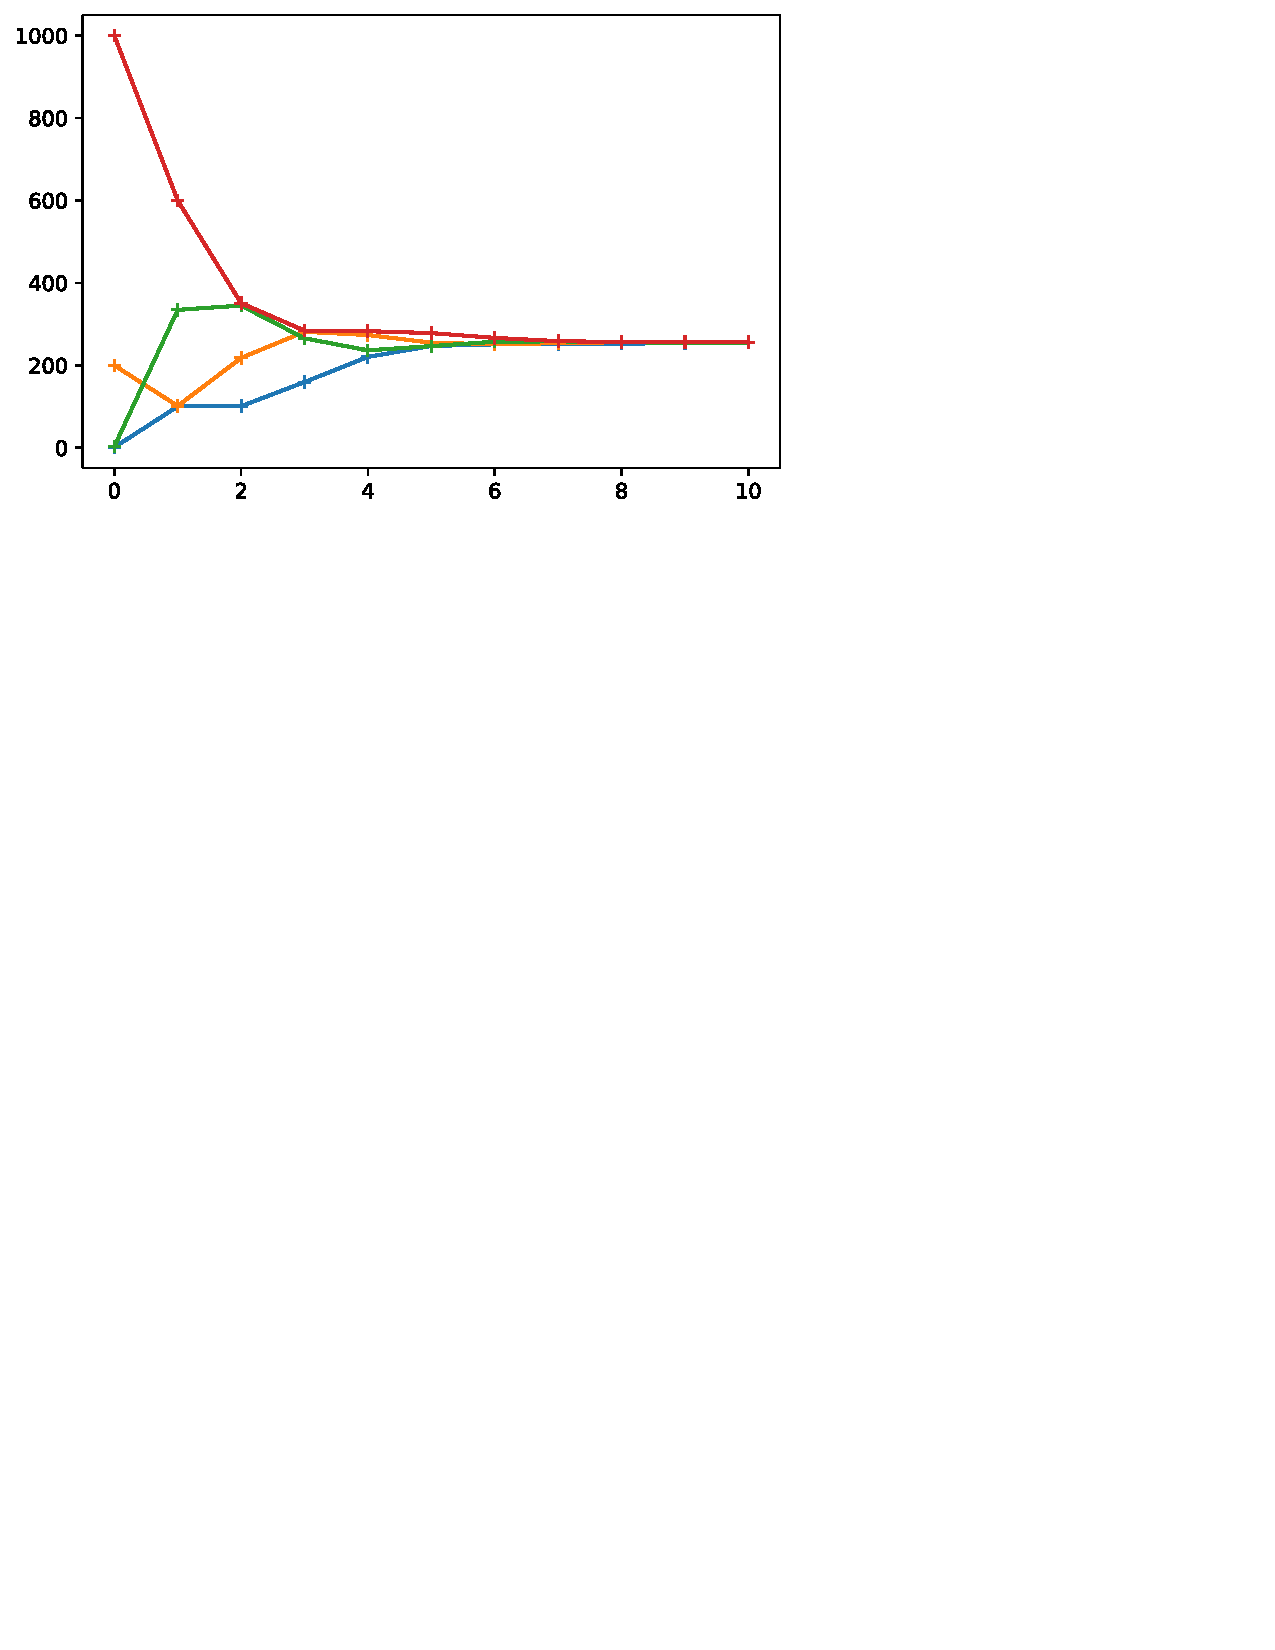
\includegraphics{1234.pdf}
    \caption{初值为1,2,3,4迭代10次的价格曲线}
    \label{fig:Result-1234}
\end{figure}

数据如表~\ref{tab:Result-1234}所示。

\begin{table}[htbp]
    \centering
    \begin{tabular}{|l|l|l|l|l|}
    \hline
    \diagbox{迭代次数}{$X_{i,j}$}{节点编号} %添加斜线表头
       & 0        & 1        & 2        & 3        \\ \hline
    0  & 1        & 2        & 3        & 4        \\ \hline
    1  & 1.5      & 2.5      & 2.666667 & 3        \\ \hline
    2  & 2        & 2.583333 & 2.388889 & 2.75     \\ \hline
    3  & 2.291667 & 2.486111 & 2.37963  & 2.666667 \\ \hline
    4  & 2.388889 & 2.43287  & 2.445988 & 2.576389 \\ \hline
    5  & 2.41088  & 2.439429 & 2.470422 & 2.50463  \\ \hline
    6  & 2.425154 & 2.454925 & 2.461977 & 2.472029 \\ \hline
    7  & 2.44004  & 2.458451 & 2.453054 & 2.463477 \\ \hline
    8  & 2.449246 & 2.455752 & 2.45219  & 2.460964 \\ \hline
    9  & 2.452499 & 2.453971 & 2.454133 & 2.458358 \\ \hline
    10 & 2.453235 & 2.454052 & 2.454997 & 2.456165 \\ \hline
    \end{tabular}
    \caption{初值为1,2,3,4迭代10次各节点价格变化}
    \label{tab:Result-1234}
\end{table}

取初值为1000,0,0,0迭代10次:

随着迭代各机组的价格曲线如图~\ref{fig:Result-1000}所示。

\begin{figure}[htbp] % use float package if you want it here
    \centering
    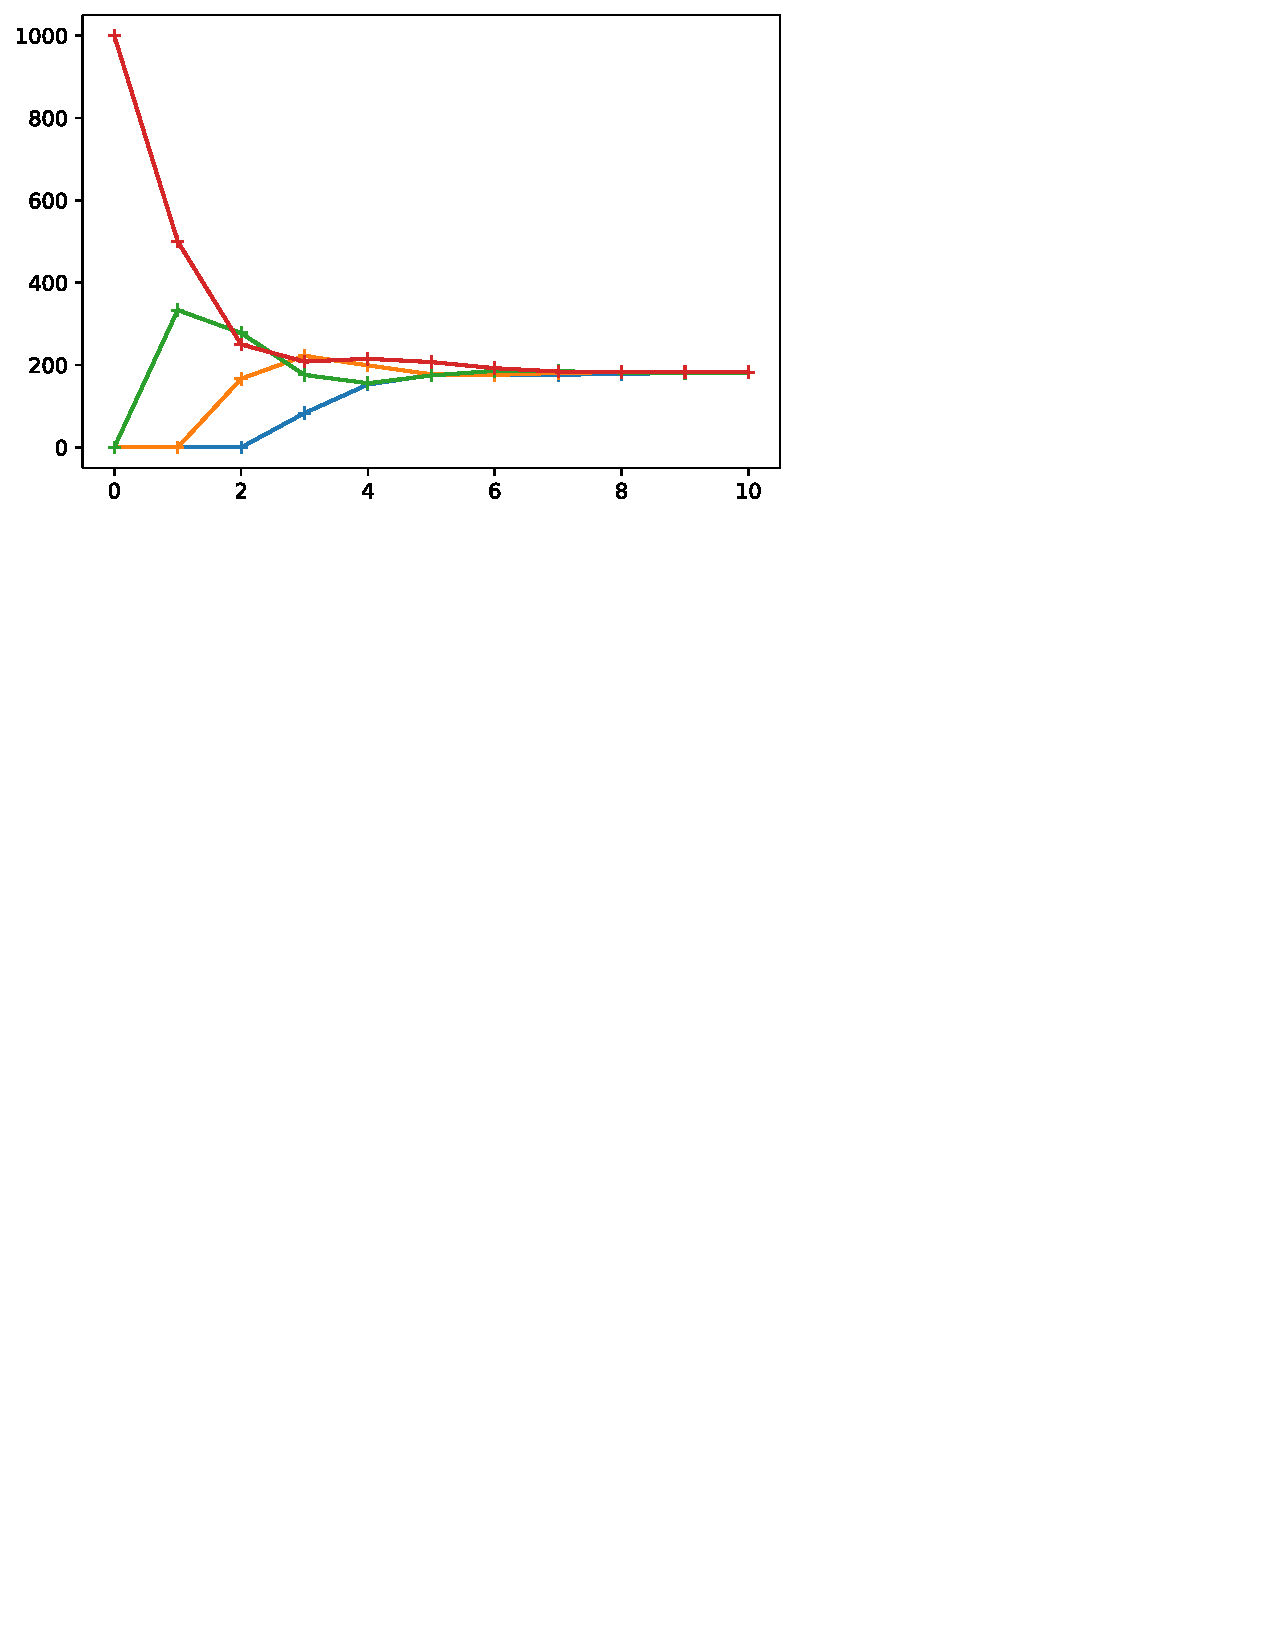
\includegraphics{1000.pdf}
    \caption{初值为1000,0,0,0迭代10次的价格曲线}
    \label{fig:Result-1000}
\end{figure}

数据如表~\ref{tab:Result-1000}所示。

\begin{table}[htbp]
    \centering
    \begin{tabular}{|l|l|l|l|l|}
    \hline
    \diagbox{迭代次数}{$X_{i,j}$}{节点编号} %添加斜线表头
       & 0        & 1        & 2        & 3        \\ \hline
    0  & 0        & 0        & 0        & 1000     \\ \hline
    1  & 0        & 0        & 333.3333 & 500      \\ \hline
    2  & 0        & 166.6667 & 277.7778 & 250      \\ \hline
    3  & 83.33333 & 222.2222 & 175.9259 & 208.3333 \\ \hline
    4  & 152.7778 & 199.0741 & 155.8642 & 215.2778 \\ \hline
    5  & 175.9259 & 177.4691 & 174.6399 & 207.1759 \\ \hline
    6  & 176.6975 & 176.0545 & 185.9139 & 192.3225 \\ \hline
    7  & 176.376  & 180.9842 & 184.978  & 184.1885 \\ \hline
    8  & 178.6801 & 182.9811 & 181.8475 & 182.5864 \\ \hline
    9  & 180.8306 & 182.4143 & 181.038  & 182.7837 \\ \hline
    10 & 181.6225 & 181.7262 & 181.5508 & 182.599  \\ \hline
    \end{tabular}
    \caption{初值为1000,0,0,0迭代10次各节点价格变化}
    \label{tab:Result-1000}
\end{table}

% \section{优化后的算法}